% ═════════════════════════════════════════════════════════════════════════════
\chapter{Implementazioni Fisiche Differenti e PC Quantistici nel Diamante}
\label{chap:implementazioni}
% ═════════════════════════════════════════════════════════════════════════════

% ─────────────────────────────────────────────────────────────────────────────
\section{Introduzione alle Piattaforme Hardware}
\label{sec:intro-hw}
% ─────────────────────────────────────────────────────────────────────────────

Realizzare fisicamente un qubit è un problema aperto e centrale della ricerca
sperimentale odierna. Qualunque sistema fisico a due livelli coerentemente
controllabile può, in linea di principio, fungere da qubit; tuttavia le
richieste pratiche sono stringenti: tempi di coerenza $T_1$ e $T_2$ lunghi
rispetto alle porte, alta fedeltà di inizializzazione e misurazione, capacità
di scaling e connettività tra qubit distinti.

I criteri formulati da DiVincenzo~\cite{divincenzo2000physical} costituiscono il
riferimento teorico condiviso: (i) sistema fisico scalabile con qubit ben
caratterizzati; (ii) inizializzazione in uno stato puro noto; (iii) tempi di
decoerenza molto più lunghi dei tempi di porta; (iv) insieme universale di
porte; (v) misurazione selettiva del qubit.

Le principali famiglie di implementazione attualmente attive sono i qubit
\textit{superconduttori}, le \textit{trappole ioniche}, i qubit \textit{fotonici},
i qubit \textit{topologici} e i \textit{centri a lacuna azotata nel diamante}
(centri NV). Le sezioni seguenti analizzano ciascuna tecnologia, con particolare
approfondimento sull'ultima, che rappresenta una delle frontiere più promettenti
per la computazione quantistica a temperatura ambiente.

% ─────────────────────────────────────────────────────────────────────────────
\section{Qubit Superconduttori}
\label{sec:supercond}
% ─────────────────────────────────────────────────────────────────────────────

\subsection{Principio fisico}
\label{subsec:sc-principio}

I qubit superconduttori sfruttano la quantizzazione dell'energia nei circuiti
LC non lineari costruiti attorno alla \textbf{giunzione Josephson}: una
sottile barriera isolante tra due strati di materiale superconduttore attraverso
la quale le coppie di Cooper possono effettuare tunnelling quantistico coerente.
La corrente critica $I_0$ della giunzione introduce una non-linearità che
separa lo spettro energetico, consentendo di isolare i soli livelli $\ket{0}$
e $\ket{1}$ come qubit computazionale.

\begin{definizione}[Giunzione Josephson]
  Una \textbf{giunzione Josephson} è un elemento di circuito superconduttivo
  formato da due elettrodi superconduttori separati da una barriera sottile
  (ossido o metallo normale). La sua energia potenziale è:
  \begin{equation}
    U(\varphi) = -E_J \cos\varphi, \qquad E_J = \frac{\hbar I_0}{2e},
  \end{equation}
  dove $\varphi$ è la differenza di fase della funzione d'onda di condensato
  tra i due elettrodi ed $E_J$ è l'energia Josephson.
\end{definizione}

Il tipo di qubit superconduttore più diffuso è il \textbf{transmon}, introdotto
da Koch \textit{et al.}~\cite{koch2007charge}: opera nel regime in cui l'energia
di carica $E_C \ll E_J$, riducendo drasticamente la sensibilità al rumore di
carica rispetto ai predecessori (charge qubit, flux qubit, phase qubit).

\subsection{Architetture e stato dell'arte}
\label{subsec:sc-stato}

IBM e Google adottano entrambe architetture planari basate su transmon. Il
processore \textit{Eagle} di IBM (127 qubit, 2021) e il già citato
\textit{Condor} (1\,121 qubit, 2023) sono connessi da risonatori bus in
topologia a griglia pesante (\textit{heavy-hex}), che riduce il tasso di
errori del two-qubit gate CNOT. Google con \textit{Sycamore} e il successivo
\textit{Willow} (105 qubit, 2024) utilizza invece una topologia a griglia
quadrata con accoppiatori sintonizzabili.

\begin{table}[ht]
  \centering
  \renewcommand{\arraystretch}{1.3}
  \caption{Parametri tipici dei qubit superconduttori (transmon, dati 2023--2024).}
  \label{tab:transmon}
  \begin{tabularx}{\textwidth}{lX}
    \toprule
    Parametro & Valore tipico \\
    \midrule
    Temperatura operativa        & $\sim 15\,\text{mK}$ \\
    Frequenza di transizione     & $4$--$8\,\text{GHz}$ \\
    Tempo di rilassamento $T_1$  & $50$--$500\,\mu\text{s}$ \\
    Tempo di sfasamento $T_2$    & $50$--$300\,\mu\text{s}$ \\
    Durata porta a 1 qubit       & $20$--$50\,\text{ns}$ \\
    Fedeltà porta a 2 qubit      & $99{,}0$--$99{,}7\,\%$ \\
    \bottomrule
  \end{tabularx}
\end{table}

Il principale svantaggio è la necessità di raffreddamento criogenico a
$\sim 15\,\text{mK}$, che richiede sistemi frigoriferi a diluizione di grande
ingombro e costo, rendendo difficile lo scaling a milioni di qubit fisici
necessari per la correzione degli errori a livello di codice di superficie.

% ─────────────────────────────────────────────────────────────────────────────
\section{Trappole Ioniche}
\label{sec:trap}
% ─────────────────────────────────────────────────────────────────────────────

\subsection{Principio fisico}
\label{subsec:trap-principio}

Nei qubit a \textbf{trappola ionica}, i livelli iperfini o ottici di ioni
intrappolati (tipicamente $^{171}$Yb$^+$, $^{40}$Ca$^+$ o $^{133}$Ba$^+$)
codificano i gradi di libertà $\ket{0}$ e $\ket{1}$. Gli ioni sono confinati da
campi elettromagnetici oscillanti (\textit{trappola di Paul}) o da campi
statici combinati (\textit{trappola di Penning}) in regioni submillimetriche
dello spazio.

Le porte logiche a singolo qubit si realizzano tramite impulsi laser o
microonde risonanti con la transizione qubit. Le porte a due qubit sfruttano
le interazioni \textit{spin-moto}: la forza di Møller-Sørensen e il gate di
Cirac-Zoller~\cite{cirac1995quantum} entanglano due ioni attraverso i modi
condivisi di oscillazione del cristallo ionico nel trap.

\subsection{Prestazioni e limitazioni}
\label{subsec:trap-presta}

I qubit a trappola ionica raggiungono le fedeltà più alte attualmente misurate:
fedeltà di porta a due qubit superiori al $99{,}9\,\%$ sono state dimostrate
con coppie di ioni~\cite{ballance2016highfidelity}. I tempi di coerenza sono
dell'ordine di secondi, fino a ore in sistemi isolati. Il limite principale è
la \textbf{velocità}: le porte a due qubit richiedono $\sim 10$--$1000\,\mu$s
a causa della mediazione attraverso i modi fononici, un ordine di grandezza
più lente rispetto ai superconduttori. La connettività è nativamente
\textit{all-to-all} (ogni ione interagisce con qualsiasi altro attraverso i
modi comuni), ma lo scaling a centinaia di qubit sulla stessa catena introduce
difficoltà nella gestione del numero di modi fononici.

Aziende come IonQ, Quantinuum (Honeywell) e Oxford Ionics stanno sviluppando
architetture a moduli multipli interconnessi da fibre ottiche per superare il
limite di scala.

% ─────────────────────────────────────────────────────────────────────────────
\section{Qubit Fotonici}
\label{sec:fotonici}
% ─────────────────────────────────────────────────────────────────────────────

I qubit \textbf{fotonici} codificano l'informazione quantistica in stati di
polarizzazione, percorso o numero di fotone. Il vantaggio fondamentale è la
\textbf{decoerenza intrinsecamente bassa}: i fotoni, privi di carica e massa,
interagiscono debolmente con l'ambiente.

L'ostacolo principale è la realizzazione di porte deterministiche a due qubit,
che richiede interazioni fotone-fotone intrinse\-camente deboli. Lo schema
KLM~\cite{knill2001scheme} (Knill-Laflamme-Milburn) dimostrò che la computazione
lineare ottica con risorse ausiliarie e misure è sufficiente per la
computazione quantistica universale, a costo di alta probabilità di successo
solo probabilistica.

Approcci più recenti sfruttano \textbf{sorgenti di fotoni singoli deterministici}
(punti quantici, centri NV) integrati in guide d'onda fotoniche su chip di
silicio o nitruro di silicio, realizzando circuiti fotonici integrati scalabili.
PsiQuantum e Xanadu puntano rispettivamente a processori fotonici
nell'infrastruttura CMOS e a varianti gaussiane (\textit{squeezed light}).

% ─────────────────────────────────────────────────────────────────────────────
\section{Qubit Topologici}
\label{sec:topologici}
% ─────────────────────────────────────────────────────────────────────────────

I qubit \textbf{topologici} codificano l'informazione in gradi di libertà
non-locali di particelle quasi-particellari chiamate \textbf{fermioni di
Majorana}, che emergono come stati a energia zero agli estremi di nanofili
superconduttori in regime topologico~\cite{kitaev2003fault}.

La caratteristica distintiva è la \textbf{protezione topologica}: le
perturbazioni locali non possono flippare il qubit, poiché l'informazione è
distribuita tra due modi di Majorana spazialmente separati. In linea di
principio questo elimina la principale fonte di decoerenza, consentendo porte
logiche \textit{fault-tolerant by design} tramite operazioni di
\textit{braiding} dei modi di Majorana.

Microsoft ha investito intensamente in questa direzione. Nel 2025 ha annunciato
una prima dimostrazione di qubit topologici con tempi di coerenza misurabili
nel sistema Majorana~1, basato su giunzioni InAs/Al. La tecnologia rimane
tuttavia alla fase dimostrativa: il controllo preciso del braiding su larga
scala costituisce una sfida ingegneristica aperta.

% ─────────────────────────────────────────────────────────────────────────────
\section{Centri NV nel Diamante}
\label{sec:nv}
% ─────────────────────────────────────────────────────────────────────────────

\subsection{Struttura e proprietà del centro NV}
\label{subsec:nv-struttura}

Il \textbf{centro a lacuna azotata} (\textit{nitrogen-vacancy centre}, NV) è
un difetto puntuale nel reticolo cristallino del diamante formato da un atomo
di \textbf{azoto} sostitutivo adiacente a una \textbf{lacuna reticolare}
(Figura~\ref{fig:nv-lattice}). La struttura presenta simmetria $C_{3v}$ e due
stati di carica dominanti: NV$^0$ (neutro) e NV$^-$ (negativamente carico).
La versione computazionalmente rilevante è NV$^-$, che ospita sei elettroni
con un sistema di spin $S = 1$.

\begin{figure}[ht]
  \centering
  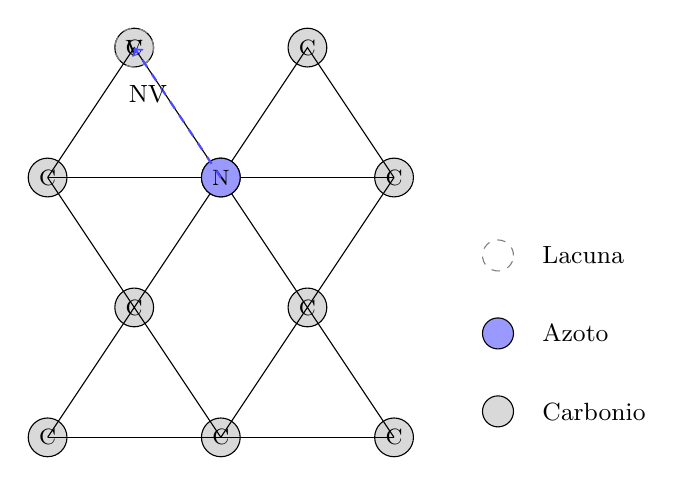
\begin{tikzpicture}[scale=1.1,
    C/.style={circle, draw=black, fill=gray!30, minimum size=14pt, inner sep=0pt},
    N/.style={circle, draw=black, fill=blue!40, minimum size=14pt, inner sep=0pt},
    V/.style={circle, draw=black!50, dashed, minimum size=14pt, inner sep=0pt}]

    % Reticolo di carboni
    \foreach \x/\y in {0/0, 2/0, 4/0, 1/1.5, 3/1.5, 0/3, 2/3, 4/3, 1/4.5, 3/4.5} {
      \node[C] at (\x,\y) {\footnotesize C};
    }

    % Legami (selezione rappresentativa)
    \draw (0,0)--(2,0)--(4,0);
    \draw (0,3)--(2,3)--(4,3);
    \draw (0,0)--(1,1.5)--(2,0);
    \draw (2,0)--(3,1.5)--(4,0);
    \draw (0,3)--(1,4.5)--(2,3);
    \draw (2,3)--(3,4.5)--(4,3);
    \draw (1,1.5)--(0,3); \draw (1,1.5)--(2,3);
    \draw (3,1.5)--(2,3); \draw (3,1.5)--(4,3);

    % Atomo di azoto (sostituisce C in 2,3)
    \node[N] at (2,3) {\footnotesize N};

    % Lacuna (adiacente all'azoto in 1,4.5)
    \node[V] at (1,4.5) {\footnotesize V};
    \draw[dashed, ->, thick, blue!70] (2,3) -- (1,4.5)
          node[midway, above left, black, font=\small] {NV};

    % Legenda
    \node[C, scale=0.8] at (5.2,0.3) {};
    \node[right, font=\small] at (5.6,0.3) {Carbonio};
    \node[N, scale=0.8] at (5.2,1.2) {};
    \node[right, font=\small] at (5.6,1.2) {Azoto};
    \node[V, scale=0.8] at (5.2,2.1) {};
    \node[right, font=\small] at (5.6,2.1) {Lacuna};
  \end{tikzpicture}
  \caption{Schema del centro NV nel reticolo cristallino del diamante. L'atomo
    di azoto sostituisce un carbonio e la lacuna occupa il sito adiacente lungo
    l'asse $\langle 111 \rangle$.}
  \label{fig:nv-lattice}
\end{figure}

\begin{definizione}[Centro NV$^-$]
  Il centro NV$^-$ è un difetto del diamante con sistema di spin $S = 1$ il
  cui stato fondamentale tripletto ($^3A_2$) presenta una scissione a campo
  zero:
  \begin{equation}
    \mathcal{H}_0 = D\left(S_z^2 - \frac{S(S+1)}{3}\right) + \gamma_e \mathbf{B} \cdot \mathbf{S},
    \label{eq:ham-nv}
  \end{equation}
  con $D \approx 2{,}87\,\text{GHz}$ parametro di separazione fine, $\gamma_e$
  rapporto giromagnetico dell'elettrone e $\mathbf{B}$ campo magnetico esterno.
\end{definizione}

\subsection{Codifica del qubit e struttura dei livelli}
\label{subsec:nv-qubit}

Il qubit è codificato nei sottostati $m_s = 0$ e $m_s = -1$ dello stato
fondamentale tripletto $^3A_2$ (Figura~\ref{fig:nv-levels}). In assenza di
campo magnetico i livelli $m_s = \pm 1$ sono degeneri a $\sim 2{,}87\,\text{GHz}$
sopra $m_s = 0$; un campo magnetico statico $B_z$ rimuove tale degenerazione
via effetto Zeeman, isolando la coppia $\{m_s = 0, m_s = -1\}$ come sistema a
due livelli ben definito.

\begin{figure}[ht]
  \centering
  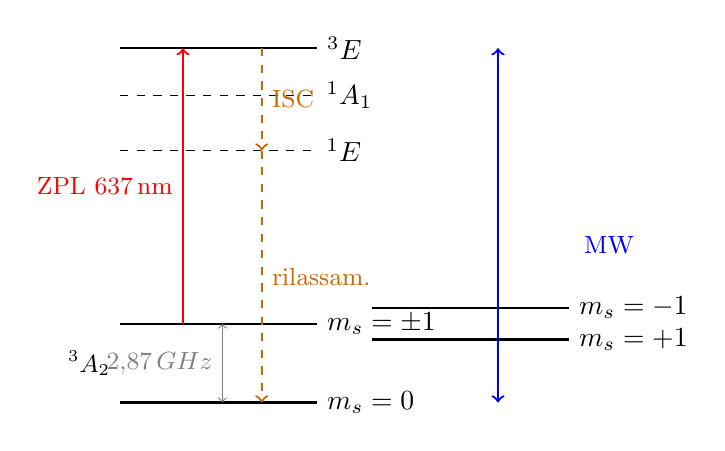
\begin{tikzpicture}[scale=1.0]
    % Stato fondamentale
    \draw[thick] (0,0) -- (2.5,0) node[right] {$m_s = 0$};
    \draw[thick] (0,1.0) -- (2.5,1.0) node[right] {$m_s = \pm 1$};
    \draw[thick] (3.2,0.8) -- (5.7,0.8) node[right] {$m_s = +1$};
    \draw[thick] (3.2,1.2) -- (5.7,1.2) node[right] {$m_s = -1$};

    % Annotazione scissione
    \draw[<->, gray] (1.3,0) -- (1.3,1.0)
          node[midway, left, font=\small] {$2{,}87\,\text{GHz}$};

    % Stato eccitato
    \draw[thick] (0,4.5) -- (2.5,4.5) node[right] {$^3E$};
    \draw[dashed] (0,3.9) -- (2.5,3.9) node[right] {$^1A_1$};
    \draw[dashed] (0,3.2) -- (2.5,3.2) node[right] {$^1E$};

    % Etichette degli stati
    \node[left, font=\small\bfseries] at (0,0.5) {$^3A_2$};
    \node[left, font=\small\bfseries] at (0,4.5) {};

    % Transizione ottica
    \draw[->, thick, red] (0.8,1.0) -- (0.8,4.5)
          node[midway, left, font=\small, red] {ZPL 637\,nm};
    \draw[->, thick, orange!80!black, dashed] (1.8,4.5) -- (1.8,3.2)
          node[midway, right, font=\small] {ISC};
    \draw[->, thick, orange!80!black, dashed] (1.8,3.2) -- (1.8,0)
          node[midway, right, font=\small] {rilassam.};

    % Porta MW
    \draw[<->, thick, blue] (4.8,0) -- (4.8,4.5);
    \node[right=2pt, blue, font=\small] at (5.7,2.0) {MW};
  \end{tikzpicture}
  \caption{Struttura dei livelli energetici del centro NV$^-$. La transizione
    ottica a 637\,nm (ZPL, \textit{zero-phonon line}) ecita il tripletto;
    il \textit{inter-system crossing} (ISC) verso il singoletto $^1A_1$
    pompa preferenzialmente la popolazione in $m_s = 0$, abilitando
    l'inizializzazione ottica del qubit.}
  \label{fig:nv-levels}
\end{figure}

\subsection{Inizializzazione, controllo e lettura ottica}
\label{subsec:nv-ottica}

Uno dei tratti distintivi del centro NV è la possibilità di
\textbf{inizializzare e leggere il qubit otticamente a temperatura ambiente}:

\begin{enumerate}
  \item \textbf{Inizializzazione.} Un impulso laser verde (532\,nm) eccita sia
    $m_s = 0$ che $m_s = \pm 1$ al tripletto eccitato $^3E$. Il canale di
    decadimento non radiativo (\textit{inter-system crossing}) verso il
    singoletto $^1A_1$ è significativamente più probabile per $m_s = \pm 1$.
    Dopo pochi cicli di pompaggio ottico, la popolazione si polarizza
    preferenzialmente in $m_s = 0$ con fedeltà $> 95\,\%$.

  \item \textbf{Controllo.} Le rotazioni del qubit sono effettuate tramite
    impulsi di microonde risonanti alla frequenza $D \pm \gamma_e B_z$
    (tipicamente $2$--$3\,\text{GHz}$ in campi magnetici dell'ordine del mT).

  \item \textbf{Lettura.} Illuminando nuovamente con il laser verde, la
    fluorescenza emessa a $637$--$750\,\text{nm}$ è più intensa per
    $m_s = 0$ rispetto a $m_s = \pm 1$ (contrasto $\sim 25$--$30\,\%$
    in singolo NV), consentendo la discriminazione degli stati tramite
    fotorilevatori a singolo fotone (SPAD o SNSPDs).
\end{enumerate}

Questo schema --- noto come \textbf{ODMR}, \textit{Optically Detected Magnetic
Resonance} --- è al cuore di tutti i protocolli di controllo del qubit NV e
di magnetometria quantistica.

\subsection{Tempi di coerenza e vantaggi operativi}
\label{subsec:nv-coerenza}

Il vantaggio più straordinario del centro NV rispetto alle altre piattaforme è
la conservazione della coerenza quantistica a \textbf{temperatura ambiente}:

\begin{itemize}
  \item $T_1$ (rilassamento spin): $\sim 1$--$6\,\text{ms}$ a $300\,\text{K}$,
    raggiungendo diversi minuti a temperature criogeniche.
  \item $T_2$ (\textit{Hahn echo}): $\sim 1$--$2\,\text{ms}$ in diamante
    ultrapuro $^{12}$C isotopicamente purificato~\cite{balasubramanian2009ultralong}.
  \item $T_2^*$ (\textit{free induction decay}): $1$--$100\,\mu\text{s}$,
    dipendente dalla densità di spin nucleari $^{13}$C nel reticolo.
\end{itemize}

La purificazione isotopica (riduzione dell'abbondanza naturale di $^{13}$C dall'1,1\%
allo $0{,}01\,\%$) ha permesso di dimostrare $T_2 > 1\,\text{s}$ su qubit
nucleari dello spin di $^{13}$C adiacenti al NV, usati come memorie
quantistiche~\cite{maurer2012room}.

\begin{notabox}
  Il qubit dello \textbf{spin nucleare} dell'atomo di azoto $^{14}$N (o
  $^{15}$N) legato al centro NV offre tempi $T_2$ ancora più lunghi rispetto
  al qubit elettronico, poiché i nuclei sono schermati dall'ambiente magnetico
  in modo più efficace. La combinazione qubit elettronico (controllo rapido) +
  qubit nucleare (memoria a lunga vita) costituisce la base delle architetture
  di ripetizione quantistica (\textit{quantum repeater}) basate su diamante.
\end{notabox}

\subsection{Integrazione cryo-CMOS: verso la scalabilità}
\label{subsec:nv-cmos}

Una delle sfide storiche dei sistemi NV è stata la distanza fisica tra i qubit
nel diamante e l'elettronica di controllo a temperatura ambiente, che causa
ritardi, rumore da cavi e difficoltà di parallelizzazione. Nel febbraio 2026,
QuTech (Delft University of Technology) ha presentato all'IEEE International
Solid-State Circuits Conference (ISSCC) la prima realizzazione di un
\textbf{chip cryo-CMOS} integrato direttamente nell'ambiente criogenico del
centro NV, capace di controllare simultaneamente spin elettronici e
nucleari~\cite{babaie2026cryogenic}.

Il sistema-su-chip sviluppato dal gruppo di Babaie e Sebastiano (Fujitsu/QuTech)
presenta adattamento digitale alla frequenza di risonanza individuale di ciascun
qubit, eliminando la necessità di sintonizzazione manuale del campo magnetico.
I risultati sperimentali ottenuti sono notevoli:

\begin{itemize}
  \item Fedeltà di porta sullo spin \textbf{elettronico}: $99{,}3\,\%$.
  \item Fedeltà di porta sullo spin \textbf{nucleare}: $99{,}8\,\%$.
  \item Tempi di coerenza: $> 50\,\text{ms}$, un ordine di grandezza superiore
    ai valori tipici a temperatura ambiente.
\end{itemize}

Questi risultati collocano il diamante criogenico con integrazione CMOS in un
regime di fedeltà competitivo con le trappole ioniche, superando il precedente
gap rispetto alle tecnologie mature. L'architettura consente controllo parallelo
di qubit multipli con consumo di potenza ridotto, requisito indispensabile per
sistemi criogenici dove ogni milliwatt di calore dissipato penalizza la
stabilità del sistema. Questo lavoro segna la \textbf{convergenza tra
ingegneria dei semiconduttori e scienza quantistica}: il diamante non è più
limitato da una catena di cavi verso l'esterno, ma beneficia di un sottosistema
di controllo integrato scalabile secondo i metodi dell'industria CMOS.

\subsection{Qubit multipli e gate entangling nel diamante}
\label{subsec:nv-multi}

L'entanglement tra due qubit NV fisicamente separati è stato dimostrato
tramite \textbf{interconnessione fotonica}: ciascun NV emette un fotone
entangled con il proprio spin; la misura congiunta dei due fotoni in un
beam-splitter (misurazione di Bell) proietta gli spin dei due NV in uno stato
di Bell, realizzando un gate entangling remoto. Questo schema costituisce il
mattone fondamentale del \textbf{quantum repeater basato su NV} e della
trasmissione sicura su reti quantistiche a fibra ottica~\cite{hensen2015loophole}.

All'interno di un singolo cristallo, centri NV adiacenti (distanza $< 10\,\text{nm}$)
possono interagire tramite accoppiamento \textbf{dipolo-dipolo magnetico},
con una costante di accoppiamento $d_\perp \sim 50\,\text{kHz}$ a $10\,\text{nm}$.
Sebbene debole, questa interazione è stata usata per dimostrare gate a due qubit
entro singoli nanocristalli di diamante.

% ─────────────────────────────────────────────────────────────────────────────
\section{Applicazioni del Diamante Quantistico}
\label{sec:nv-applicazioni}
% ─────────────────────────────────────────────────────────────────────────────

La piattaforma NV-diamante non si limita alla computazione; le sue eccezionali
proprietà la rendono competitiva in un ampio spettro applicativo:

\begin{itemize}
  \item \textbf{Magnetometria nanoscalare.} La sensibilità al campo magnetico del
    qubit elettronico consente misure con sensibilità $\eta_B \sim 1\,\text{pT/Hz}^{1/2}$
    a temperature ambiente con risoluzione spaziale $< 10\,\text{nm}$, aprendo la
    strada all'imaging di correnti neuronali in singole cellule~\cite{degen2017quantum}.

  \item \textbf{Reti quantistiche.} Il centro NV emette fotoni nel visibile
    (637\,nm ZPL) che possono essere resi compatibili con le finestre a bassa
    perdita delle fibre ottiche tramite conversione di frequenza. Diversi
    esperimenti hanno dimostrato distribuzione di entanglement su fibre di
    1,3\,km~\cite{hensen2015loophole}.

  \item \textbf{Memoria quantistica.} I qubit nucleari dei $^{13}$C vicini al NV
    fungono da memoria quantistica con tempi di storage $\sim 1\,\text{s}$,
    utili come buffer nei quantum repeater.

  \item \textbf{Quantum sensing biomedicale.} Diamanti nanoparticellari
    contenenti NV possono essere introdotti in cellule viventi per imaging
    magnetico intracellulare non invasivo.
\end{itemize}

% ─────────────────────────────────────────────────────────────────────────────
\section{Confronto Sistematico delle Tecnologie}
\label{sec:confronto-hw}
% ─────────────────────────────────────────────────────────────────────────────

La Tabella~\ref{tab:hw-confronto} confronta le principali piattaforme hardware
lungo le dimensioni più rilevanti per la scalabilità verso la computazione
fault-tolerant.

\begin{table}[ht]
  \centering
  \renewcommand{\arraystretch}{1.3}
  \caption{Confronto delle principali piattaforme di qubit fisici (dati 2023--2025).}
  \label{tab:hw-confronto}
  \begin{tabularx}{\textwidth}{>{\bfseries}lXXXXX}
    \toprule
    Caratteristica &
    Supercondutt. &
    Trappola ionica &
    Fotonico &
    Topologico &
    NV diamante \\
    \midrule
    Temperatura op.    & 15\,mK       & Amb./UHV  & Amb.     & 15\,mK   & Amb./Cryo \\
    $T_2$ tipico       & 0.1--1\,ms   & 1\,s      & N/A*     & TBD      & 1--2\,ms (amb.) $>$50\,ms (cryo) \\
    Fedeltà 2-qubit    & 99.0--99.7\% & 99.9\%    & Variab.  & TBD      & 99.3--99.8\%$^\dagger$ \\
    Velocità porta     & 10--100\,ns  & 1--1000$\mu$s & ps--ns & Bassa  & $\mu$s \\
    Connettività       & Locale       & All-to-all & Retic.   & Locale   & Locale/Rem. \\
    Scalabilità        & Alta         & Media      & Alta     & Potenz.  & Bassa \\
    Controllo          & MW/RF        & Laser/MW   & Ottrico  & Braid.   & Laser+MW \\
    \bottomrule
    \multicolumn{6}{l}{\footnotesize *Il fotone è il qubit; $T_2$ del portatore fisico non è la figura rilevante.} \\
    \multicolumn{6}{l}{\footnotesize $^\dagger$Risultato cryo-CMOS integrato (QuTech/ISSCC 2026~\cite{babaie2026cryogenic}).}
  \end{tabularx}
\end{table}

Nessuna singola tecnologia domina tutte le dimensioni. I qubit superconduttori
guidano in velocità e integrazione su chip; le trappole ioniche in fedeltà e
coerenza; i sistemi NV nel diamante in operabilità a temperatura ambiente e
sensing. L'approccio \textbf{ibrido} --- in cui diverse piattaforme svolgono
ruoli complementari (es.\ processore superconduttore + memoria NV + link
fotonico) --- è considerato dalla comunità scientifica come il percorso più
realistico verso reti quantistiche distribuite fault-tolerant.

% ─────────────────────────────────────────────────────────────────────────────
\section{Conclusioni del Capitolo}
\label{sec:conclusioni-hw}
% ─────────────────────────────────────────────────────────────────────────────

Questo capitolo ha presentato le principali piattaforme hardware per la
realizzazione di qubit fisici, analizzando i compromessi tecnici di ciascuna.
I qubit superconduttori dominano la scena dei processori integrati grazie alla
velocità e alla compatibilità CMOS; le trappole ioniche offrono fedeltà
insuperabili ma velocità minori; i qubit fotonici sono intrinsecamente adatti
alle comunicazioni quantistiche; i qubit topologici promettono protezione
intrinseca ma rimangono tecnologicamente immaturi.

I centri NV nel diamante occupano una nicchia unica: \textbf{qubit solidi a
temperatura ambiente} con tempi di coerenza di millisecondi, manipolabili
otticamente con strumentazione relativamente accessibile. Con l'avvento
dell'integrazione cryo-CMOS (QuTech, ISSCC 2026~\cite{babaie2026cryogenic}),
la fedeltà dei gate nel diamante criogenico ha raggiunto il 99{,}3--99{,}8\,\%
con tempi di coerenza superiori a 50\,ms, colmando il divario rispetto alle
trappole ioniche. Questa convergenza tra fisica dei difetti nel diamante e
ingegneria CMOS apre la strada a processori NV scalabili su larga scala, non
più limitati dalla catena di cavi verso l'esterno.

Il capitolo successivo esaminerà gli algoritmi quantistici più rilevanti e
la loro implementazione concreta sulle piattaforme hardware descritte.